% declare what packages you use:
\documentclass[12pt]{article}
\usepackage[utf8]{inputenc}
\usepackage{amsmath}
\usepackage{amssymb}
\usepackage{amsthm}
\usepackage{enumitem}
\usepackage{mathtools}
\usepackage[letterpaper]{geometry}
\geometry{margin=0.8in}
\usepackage{hyperref}

% The title of the report
\title{Comp 251 Proofs Assignment Report}
% Write your name in author
\author{Lucas Chew, 260971542 \and No Collaborators }
% Course code and date
\date{Comp251, Winter 2023}



\begin{document}
\maketitle

% Report the first claim you will prove here
\section*{Claim 1}
Deleting a node x from an AVL tree takes O(log n) time.

% Report the proof of the claim here
\section*{Proof}
This proof is adapted from Cormen, Leiserson, Rivest, and Stein, \textit{Introduction to Algorithms} \cite{cormen2009introduction}.
\begin{proof}
There are $3$ components of the Bellman-Ford Algorithm that we can reason about individually.
\begin{enumerate}
    \item \textsc{Initialize-Single-Source(G,s)}
    In this function we iterate through each vertex of the graph once doing constant time work each time as we are only initializing two fields for each vertex: the distance from the source vertex $s$ and the predecessor vertex on the shortest path. These are initialized as infinity and null respectively. The only exception is the distance from $s$ to $s$ is set at $0$. This takes $\Theta(V)$ time. 
    \item After initialization we do $|V|-1$ iterations, each time relaxing every edge in the graph. The relax method takes $O(1)$ time as we are doing comparisons of numerical values, and updating fields. We update the shortest path and predecessor of a vertex if we find a shorter path by taking a particular edge. Since on each of the $\Theta(V)$ iterations, we iterate through every edge exactly once, doing constant time operations, the total time of this step is $\Theta(V \cdot E)$. There is no early stopping condition in this loop, therefore it is a tight bound.  Since we are looking for a shortest path, we only iterate up to $|V|-1$ as a shortest path can only contain $|V|-1$ edges before it contains a cycle.
    \item After the main loop, we examine our final values for negative weight cycles. This process involves iterating again through every edge in the graph, doing constant time comparisons. We check if the distance to the end vertex of an edge has a larger distance than the start vertex of the edge plus the value of taking the edge, and in this case return false immediately as this corresponds to a negative cycle. Therefore, this takes $O(E)$ time. It is not $\Omega(E)$ as in the best case we find a negative weight cycle quickly and can return that one exists immediately. 
\end{enumerate}
So, the total running time is then $\Theta(V \cdot E)$. Note again that this is a tight bound as in component $2$, we always iterate through the $E$ edges, $\Theta(V)$ times.

\end{proof}

% Report the summary of the proof here
\section*{Proof Summary}
We argue the running time of each of the three main components in the algorithm. Initializing the graph vertices takes linear time as we visit each vertex exactly one once. The main for loop iterates through the number of vertices, and each iteration it iterates  through all the edges in the graph, seeing if using that edge leads to a shorter cost path. Note, that we iterate through the number of vertices because the longest, non-cyclic path can visit at most all the vertices in the graph. Finally, we iterate over the edges once again to check for a cycle. Therefore, the total run time is dominated by the iteration that repeats for the number vertices and each time iterates through all the edges. 

% Report the algorithm and java code here, including any relevant figures
\section*{Algorithm}
Below is the Java code for the Bellman-Ford shortest path method (Figure \ref{bellman-ford}, Lines 24-42). I created the data structures needed for the algorithm. This includes the classes Vertex (Figure 2), Edge (Figure 3), Graph (Figure 4), and EdgeFunction (Figure 5).  The initialize-single-source method is not needed in this variation of the algorithm as I initialize a vertex correctly when it is constructed (Figure 2, Lines 5-6). All that is necessary is to update the distance from the selected source vertex to be $0$ (Figure 1, Line 26). 

I time the execution of the Bellman-Ford algorithm when run on random graphs with $n$ vertices and $2n$ edges. I start $n$ at $10$ and then increase it by $10$ for each new instance. In total, I time the execution for up to $n=1000$. The execution time is reported in microseconds. The plot below (Figure 6) shows the execution time as a function of the number of vertices, $n$. We expect the execution time to be quadratic in $n$ ($V\cdot E = 2n^2$), and to be a tight bound. The graph confirms this claim. It can be closely modelled by the quadratic function of $n$ shown. 

The random graphs are created by creating a random path of length $n-1$ so that it is connected. The remaining edges are then added randomly. In addition, I generate a random weight function for each set of edges that assigns a nonzero weight in the range $(-100,100)$ to the edge. 

\begin{figure}[h]
  \centering
    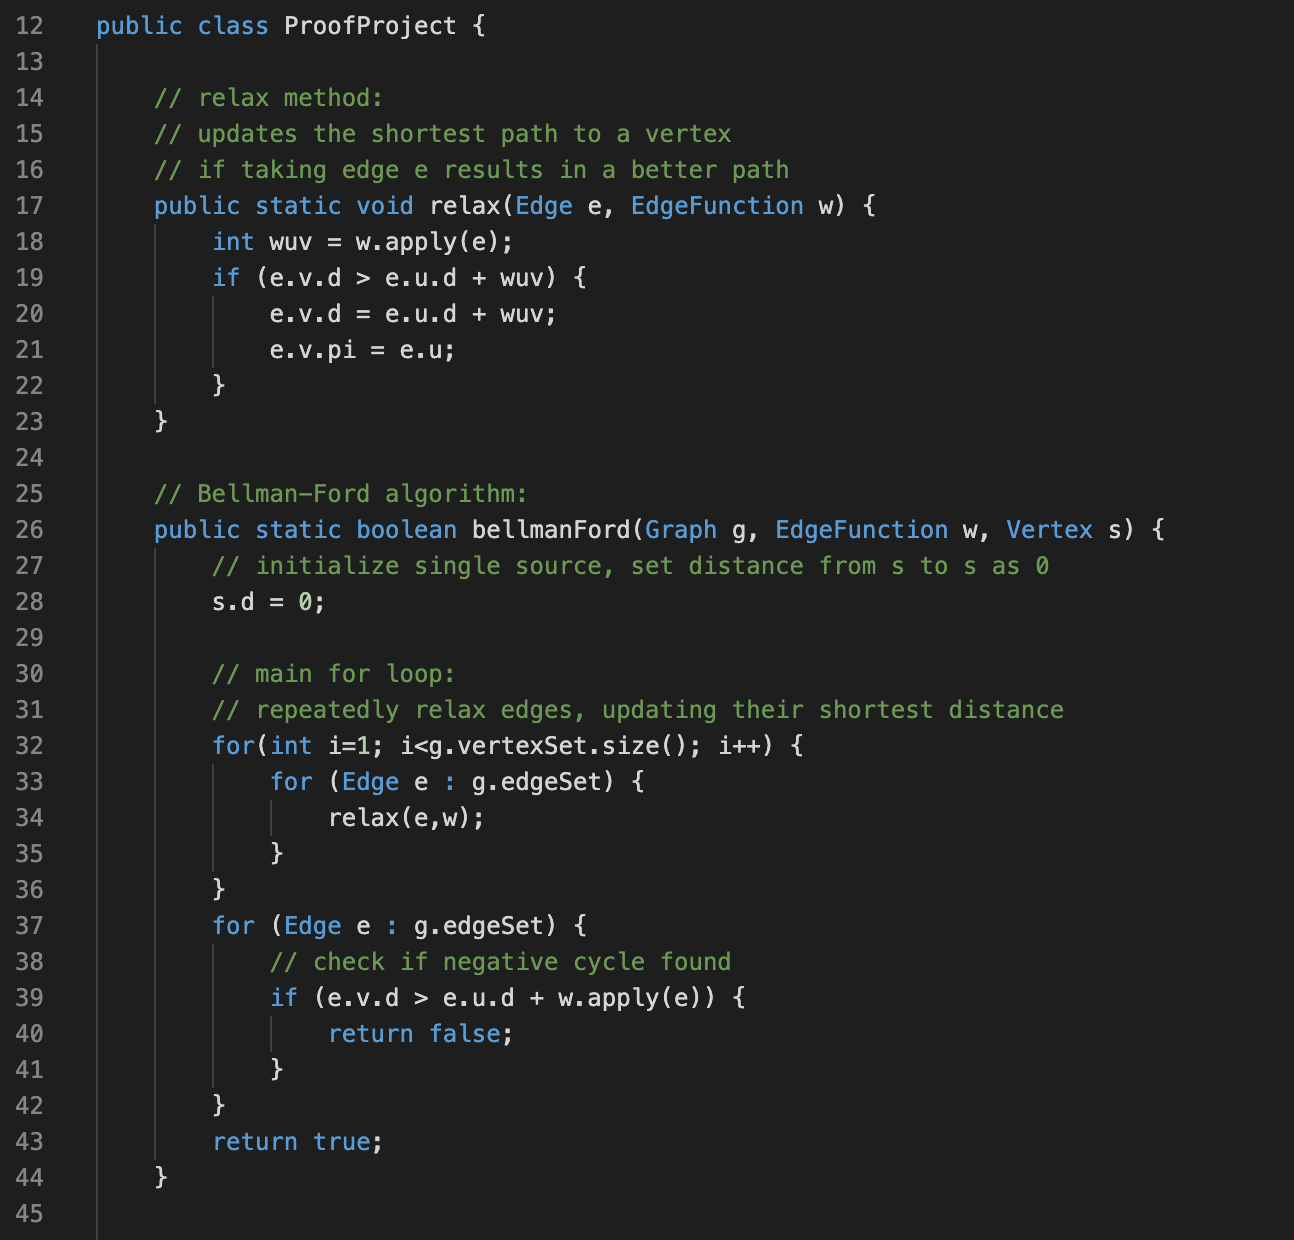
\includegraphics[scale=.5]{figures/bellman-ford.png}
    \caption{The Bellman-Ford Algorithm from \texttt{ProofProject.java}.}
    \label{bellman-ford}
\end{figure}

\begin{figure}[h]
  \centering
    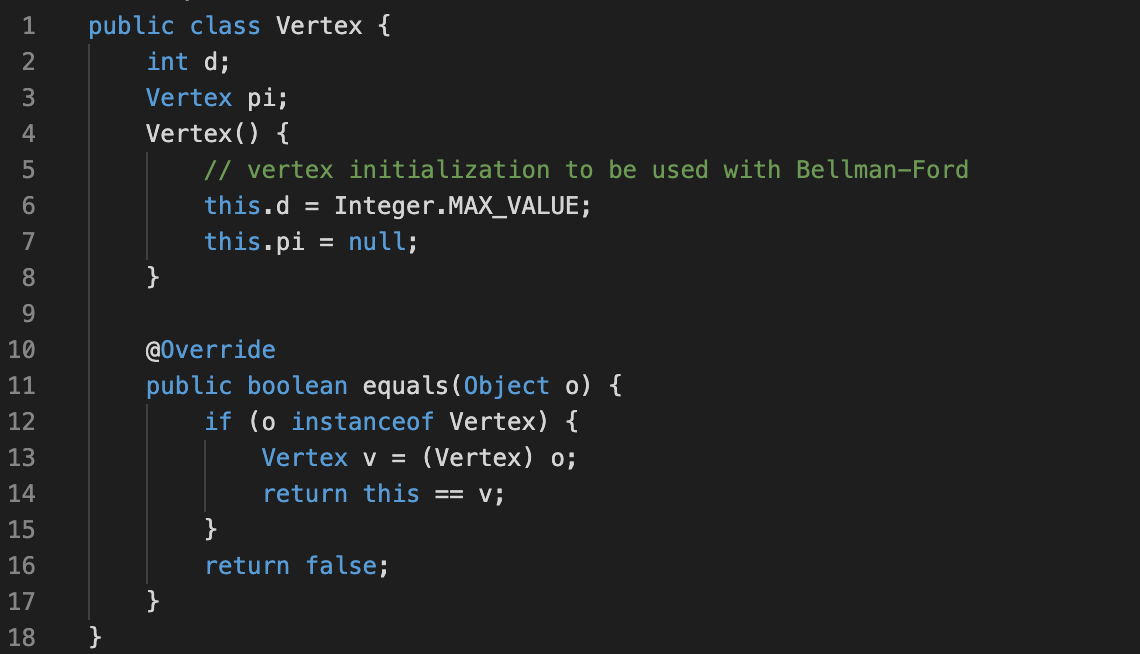
\includegraphics[scale=.5]{figures/vertex.png}
    \caption{Vertex class from \texttt{Vertex.java}.}
\end{figure}

\begin{figure}[h]
  \centering
    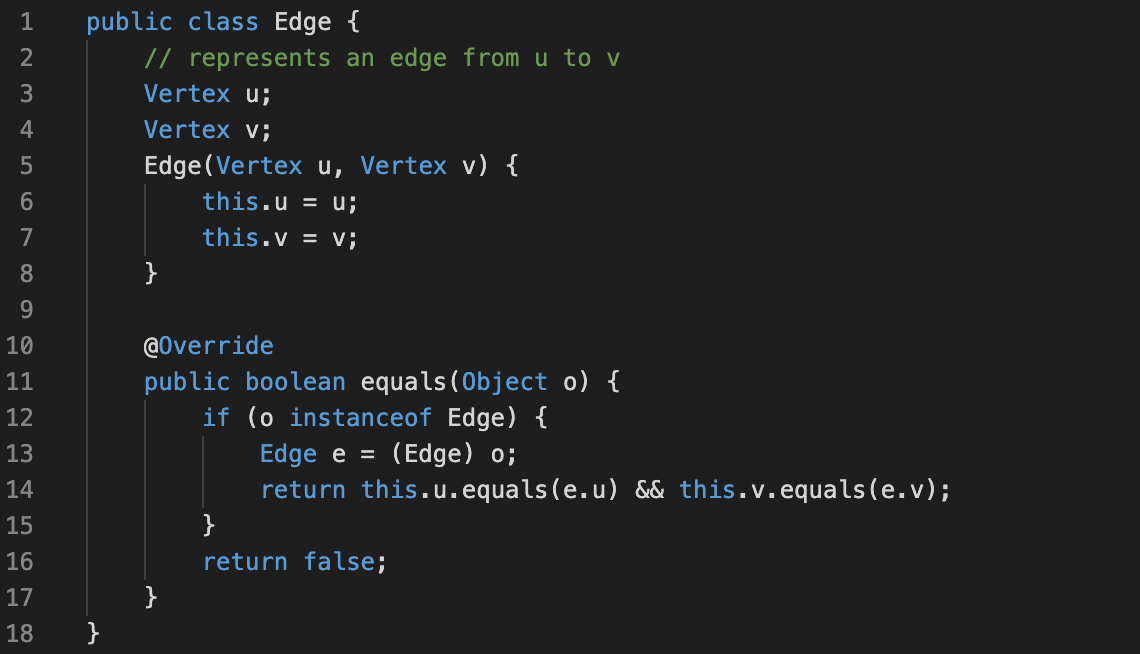
\includegraphics[scale=.5]{figures/edge.png}
        \caption{Edge class from \texttt{Edge.java}.}
\end{figure}

\begin{figure}[h]
  \centering
    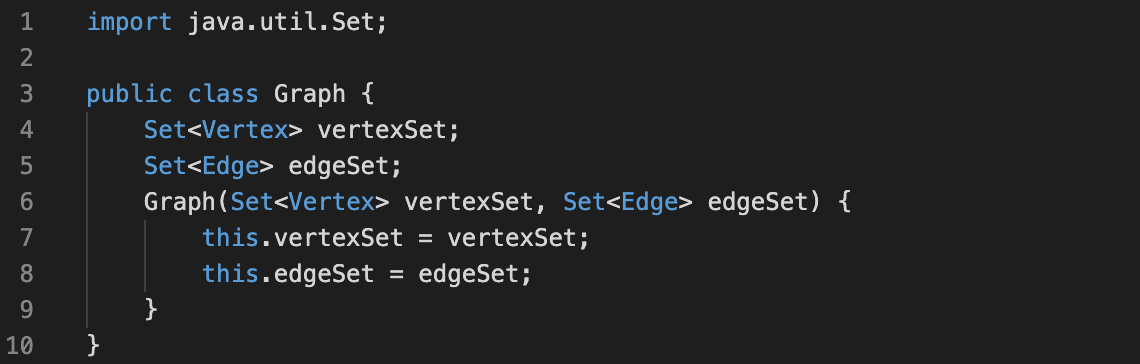
\includegraphics[scale=.5]{figures/graph.png}
        \caption{Graph class from \texttt{Graph.java}.}
\end{figure}

\begin{figure}[h]
  \centering
    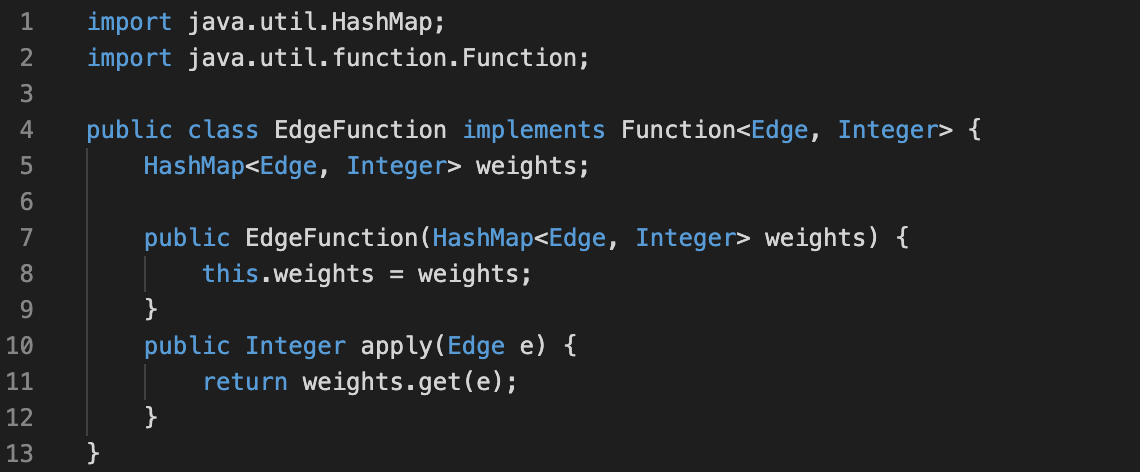
\includegraphics[scale=.5]{figures/function.png}
        \caption{EdgeFunction class from \texttt{EdgeFunction.java}.}
\end{figure}

\begin{figure}[h]
  \centering
    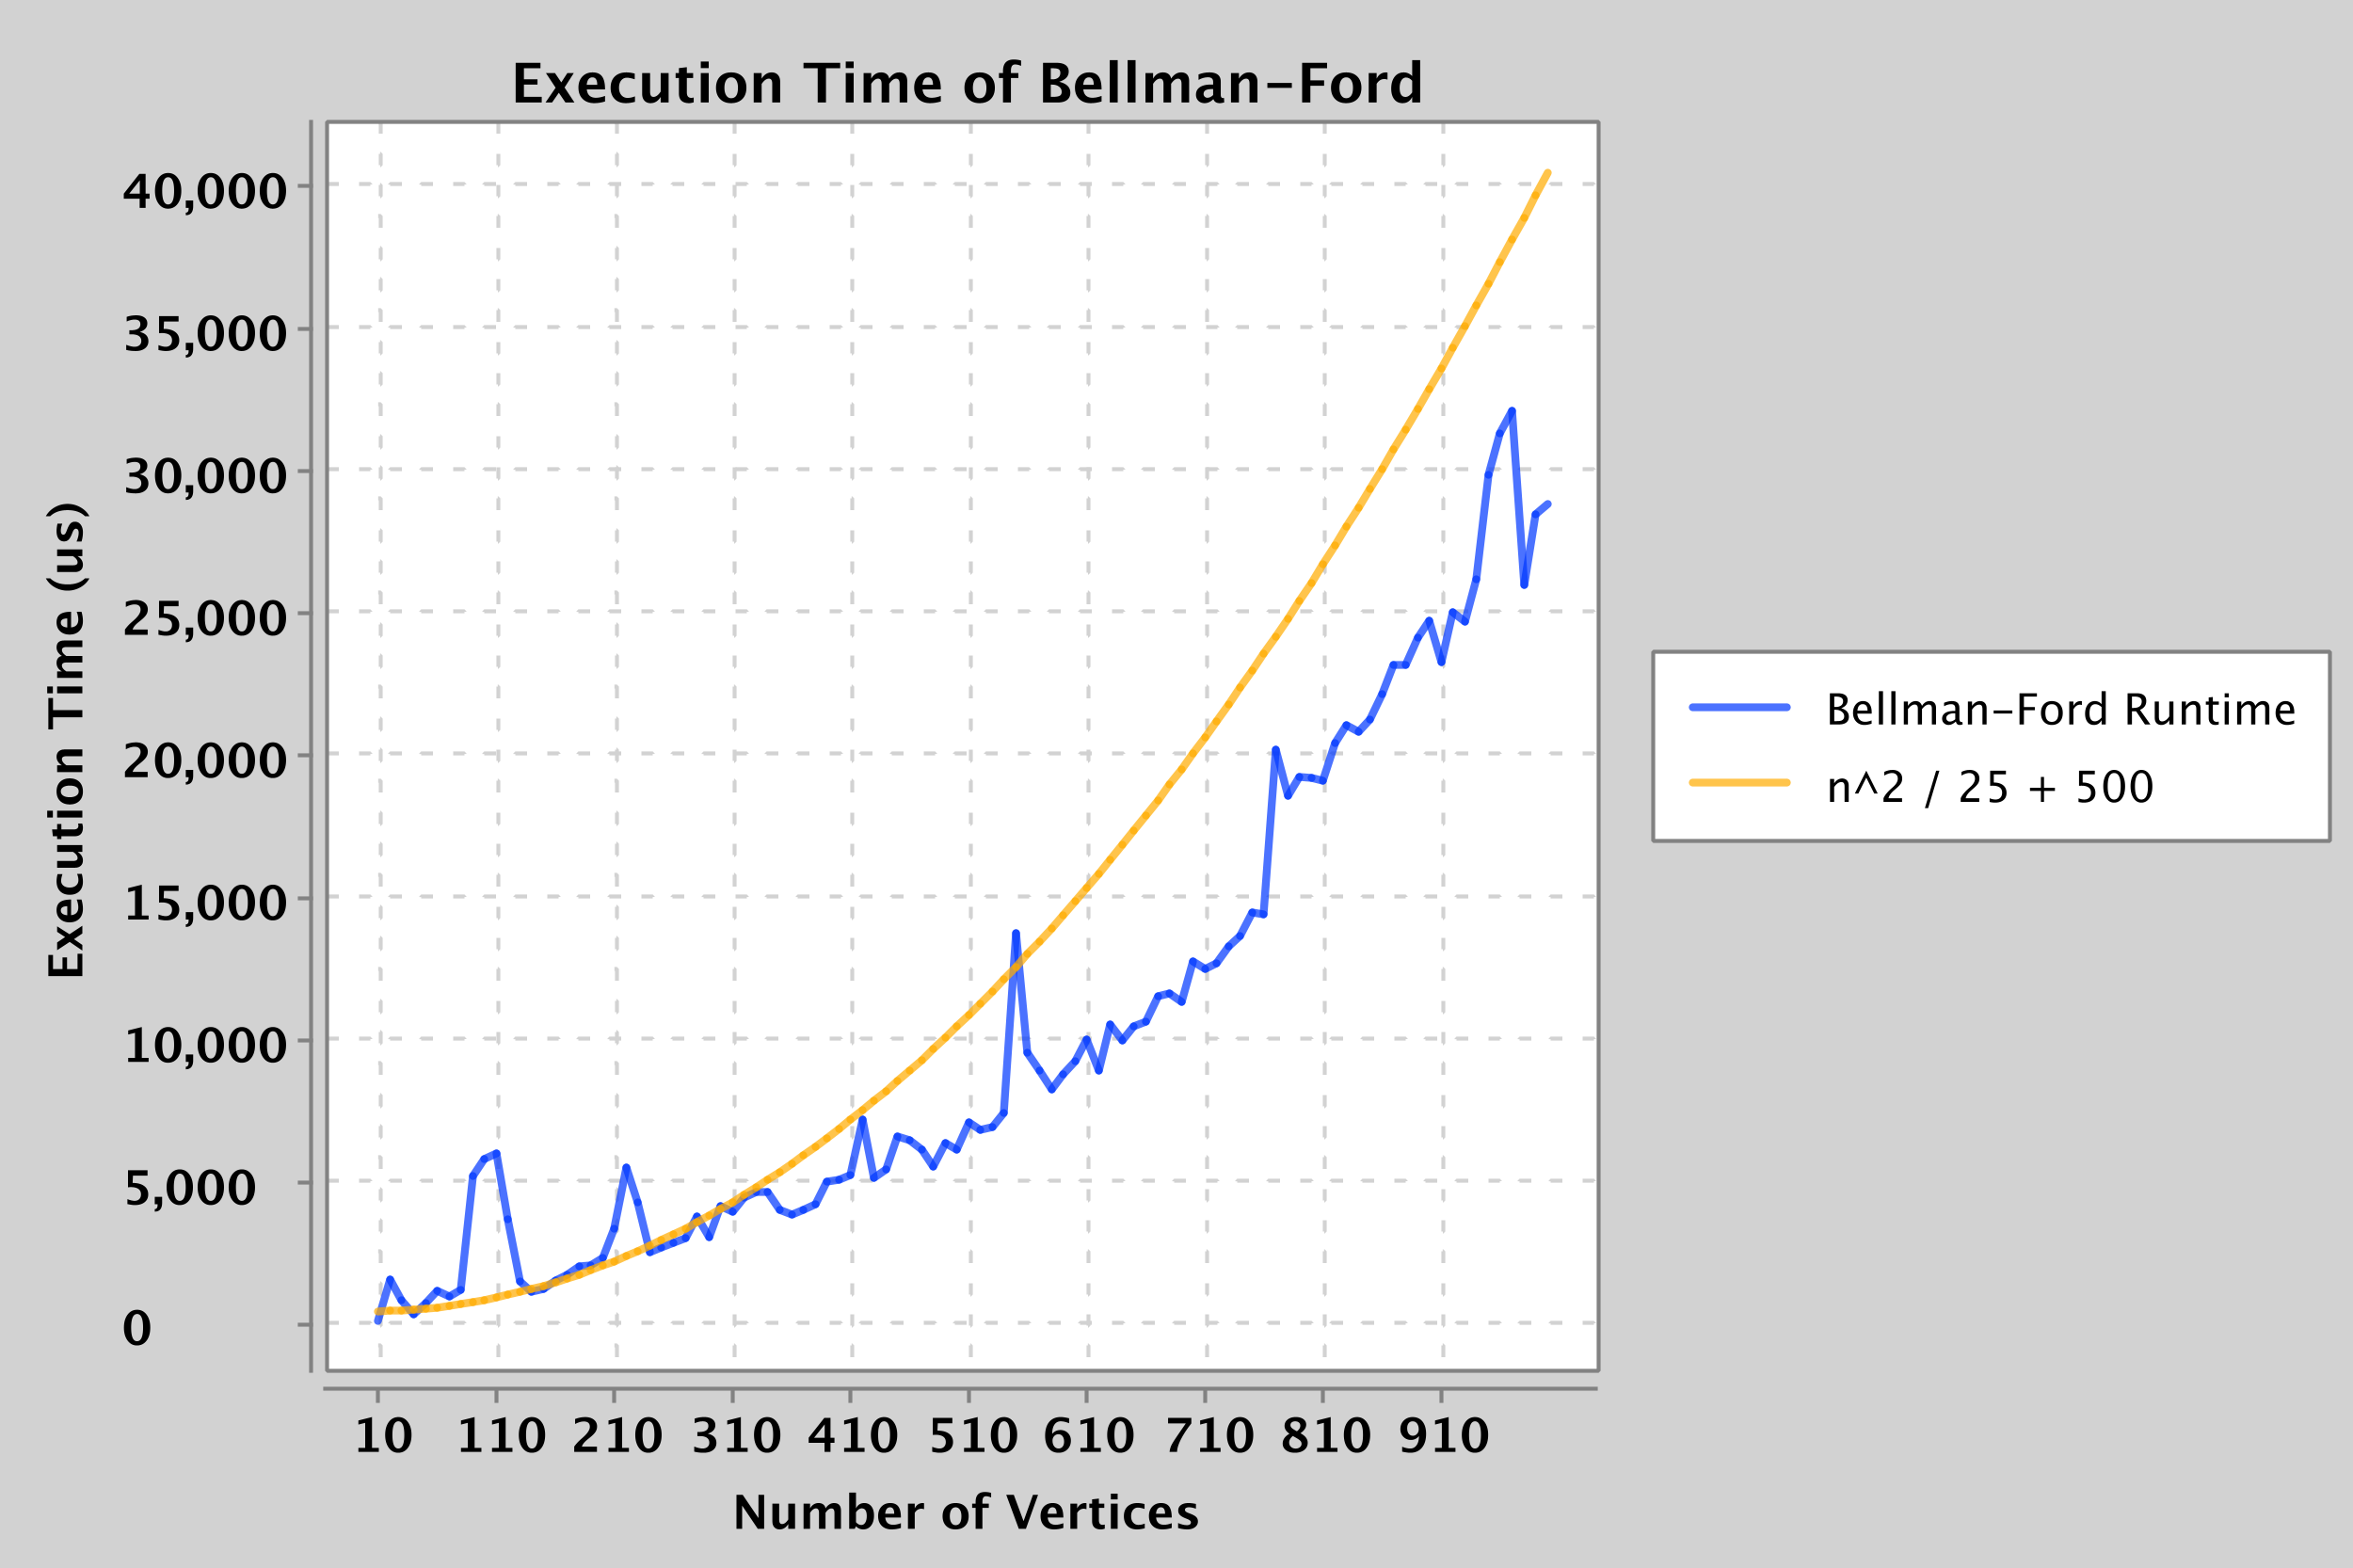
\includegraphics[scale=.5]{figures/runtime.png}
        \caption{Execution time in microseconds of Bellman-Ford as a function of $n$. The code to generate this graph is in \texttt{ProofProject.java}.}
\end{figure}

\clearpage
% Report the real world application here
\section*{Real World Application} 
The Bellman-Ford algorithm finds the shortest path in a directed graph that may contain negative weight cycles. This can be applied to any formulation of the shortest path problem. A useful application is data routing on a network, including many internet protocols. The goal is to send information through a network of routers as quickly as possible. We represent the network as a graph where vertices correspond to distributors in the network and the edges are links between distributors. The cost of an edge is the expected delay of sending information through that route. The Bellman-Ford algorithm can find the optimal route to send a packet of data from one vertex to the other as to minimize the delay. This example is from \textit{Brilliant Math \& Science Wiki}\cite{brilliant}.



\newpage
% Report the second claim you will prove here
\section*{Claim 2}
The \textsc{Dijkstra’s algorithm}, ran on a weighted, directed graph
$G = (V,E)$ with non-negative weight function $w$ and source $s$, terminates with $u.d = \delta(s, u)$
for all vertices $u \in V$.

\section*{Proof}
This proof is a paraphrased version of the proof written in \cite{cormen2009introduction}, page 680-682.  \hfill \break
Let $S$ be the initial empty set of vertices and $Q$ be the initial set of vertices will all of $G$'s vertices
We can prove this through contradictions by assuming that that a vertex $u$, does not follow the rule of $u.d != \delta(s, u)$ when adding $u$ to $S$. From this we can assume three things:

\begin{enumerate}
    \item $u \neq s$ as $u.d = s.d = 0$ would break the assumption, as $\delta(s, s) = 0$.
    \item A path $p$ exists between $u$ and $s$, as without so $\delta(s, u) = \infty$ and $u.d = \infty$ at the time of insertion, breaking our assumption.
    \item $u$ will be selected out of order, where at least one of the connected nodes is relaxed, as not doing so would make $u.d = \delta(s, u)$.
\end{enumerate}
From this, let $x, y \in V$, where $x \in S$ and $y \in Q$. Let $p1, p2 \in E$, where $p1$ connects $s$ to $x$ and $p2$ connects $y$ to $u$. \hfill \break
Let $y$ be the predecessor vertex to $u$ and be the shortest-path between $s$ and $u$. Let $x$ be the predecessor vertex to $y$. \hfill \break
As $x \in S$, we can assume that $x.d = \delta(s, x)$ and that the $Relax(x, y)$ has occurred, filling a value into $y.d$. As $u$ is the first vertex to make the assumption of $u \neq \delta(s, y)$, we can assume that $y.d = \delta(s, y)$. As $y$ is the predecessor vertex to $u$ and that the weights are non-negative, we can assume that $\delta(s, y) \le \delta(s, y)$. Therefore, this creates $y.d = \delta(s, y) \le \delta(s, u) \le u.d$. \hfill \break
If we let $u$ be the next node taken from $EXTRACT_MIN(Q)$, that would mean that $u.d <= y.d$. \hfill \break
From those two, we can use the upper-bound limits and find that $y.d = \delta(s, y) = \delta(s, u) = u.d$. This breaks our contradiction of $u.d \neq \delta(s, u)$, which should then be proven true for all subsequent cases $v.d = \delta(s, v)$ upon $v$ being inserted into $S$, $v \in V$. Therefore, upon termination of Dijkstra’s algorithm, all $v.d = \delta(s, v)$, $v \in V$.


\section*{Proof summary}
The core concept of the proof is that a vertex's distance is the smallest is can possibly be when entering the "visited" set of vertices. This is proven by assuming that a vertex's distance from the source node is not the smallest it can be, creating a contradiction. From this, we can assume that the vertex is not the source vertex, there has to be a path, and that this can only happen if that specific vertex is picked out of order, as these all break the contradiction immediately. \hfill \break
If there is a vertex before the contradiction vertex, then the contradiction vertex's distance from the source is at least greater or equal to the distance of the previous vertex, assuming that all weights are positive. However, if the contradiction vertex is picked from the priority queue before vertex before it, it would mean that the previous vertex has an equal or greater distance from the source from the contradiction vertex. Using the upper-bounds of both, we can prove an equality that the contradiction vertex's distance from source at the time of insertion into the "visited" set, is the smallest it can be.

\section*{Algorithm}
Below is the Java code for finding the shortest path using Dijkstra's Algorithm (Figure 7). The implementation required many basic classes, including Vertex (Figure 8), Edge (Figure 9), and Graph (Figure 10).

The main function ran the algorithm on three test cases, one being general and the other two being edge cases. The construction of the test cases are shown in Figure 11 and the output of the test cases are in Figure 12.

The general case contained four vertices $\{1, 2, 3, 4\}$ as well as five edges connecting them $\{(1, 2, 3), (1, 3, 5), (2, 3, 1), (2, 4, 6), (3, 4, 1)\}$ in the format: (starting vertex, ending vertex, weight). This case is clear as the shortest path is to go from index $\{1 -> 2 -> 3 -> 4\}$, gathering a total of $3+1+1 = 6$ weight.

The next edge case is the empty edge case, $E=\{\}$, and there is only one vertex, the source vertex, in this case $\{1\}$. The expected and observed output is for the source vertex to be at a weight of zero.

The last edge case is when there is a Vertex that is not connected by any edges. The vertices are $\{1, 2, 3, 4\}$ and the edges are $\{(1, 2, 3), (1, 3, 5), (2, 3, 1)\}$, where vertex index four is not connected. In this case, the output is the shortest path to each vertex, except for index four, where the distance from the source node is the maximum integer allowed, which represents $\infty$.

\clearpage
\begin{figure}[h]
    \centering
    \includegraphics[scale=0.75]{figures/Dijkstra.png}
    \caption{Algorithm for finding the shortest-path in a graph from \texttt{Dijkstra.java}.}
\end{figure}

\begin{figure}[h]
    \centering
    \includegraphics[scale=1]{figures/Vertex.png}
    \caption{Vertex class from \texttt{Vertex.java}.}
\end{figure}

\begin{figure}[h]
    \centering
    \includegraphics[scale=1]{figures/Edge.png}
    \caption{Edge class from \texttt{Edge.java}.}
\end{figure}

\begin{figure}[h]
    \centering
    \includegraphics[scale=.8]{figures/Graph.png}
    \caption{Graph class from \texttt{Graph.java}.}
\end{figure}

\begin{figure}[h]
    \centering
    \includegraphics[scale=.8]{figures/Test Cases.png}
    \caption{Functions to create general and edge test cases for Dijkstra's algorithm from \texttt{Dijkstra.java}.}
\end{figure}

\begin{figure}[h]
    \centering
    \includegraphics[scale=1]{figures/Output.png}
    \caption{Console output after running the \textsc{findShortestPath} method on the three test cases.}
\end{figure}


\clearpage
\section*{Real World Application}
This algorithm can be used to find the single-sourced shortest path on weighted, directed graphs, where the edges only contain non-negative numbers by finding the lowest non-visited vertex and adding it's connected vertices to the queue (\cite{cormen2009introduction} pages 679). A real-world example of Dijkstra's Algorithm would be the digital mapping services, like Google Maps, to find directions and a path to a location within the shortest amount of time possible. As there are many paths and methods to get to a single location, Dijkstra's Algorithm can be used to find the shortest path whether it be by walking, by public transport, or by car \cite{GeekforGeeks}.


\clearpage
% Creates bibliography (if using bibtex)
\bibliographystyle{plain}
\bibliography{myref.bib}

\end{document}
